\documentclass[aspectratio=43]{beamer}
% \documentclass[aspectratio=169]{beamer}

% Title --------------------------------------------
\title{Smart Literature Search}
\subtitle{A short intro to Litmaps, Connected Papers and Inciteful}
\date{\today}
\author{Tao Wang (JHU)}

% xcolor and define colors -------------------------
\usepackage{xcolor}

% https://www.viget.com/articles/color-contrast/
\definecolor{purple}{HTML}{5601A4}
\definecolor{navy}{HTML}{0D3D56}
\definecolor{ruby}{HTML}{9a2515}
\definecolor{alice}{HTML}{107895}
\definecolor{daisy}{HTML}{EBC944}
\definecolor{coral}{HTML}{F26D21}
\definecolor{kelly}{HTML}{829356}
\definecolor{cranberry}{HTML}{E64173}
\definecolor{jet}{HTML}{131516}
\definecolor{asher}{HTML}{555F61}
\definecolor{slate}{HTML}{314F4F}

% Main theme colors
\definecolor{accent}{HTML}{107895}
\definecolor{accent2}{HTML}{9a2515}


% Beamer Options -------------------------------------

% Background
\setbeamercolor{background canvas}{bg = white}

% Change text margins
\setbeamersize{text margin left = 15pt, text margin right = 15pt} 

% \alert
\setbeamercolor{alerted text}{fg = accent2}

% Frame title
\setbeamercolor{frametitle}{bg = white, fg = jet}
\setbeamercolor{framesubtitle}{bg = white, fg = accent}
\setbeamerfont{framesubtitle}{size = \small, shape = \itshape}

% Block
\setbeamercolor{block title}{fg = white, bg = accent2}
\setbeamercolor{block body}{fg = jet, bg = jet!10!white}

% Title page
\setbeamercolor{title}{fg = jet}
\setbeamercolor{subtitle}{fg = accent}

%% Custom \maketitle and \titlepage
\setbeamertemplate{title page}
{
    %\begin{centering}
        \vspace{20mm}
        {\Large \usebeamerfont{title}\usebeamercolor[fg]{title}\inserttitle}\\
        {\large \itshape \usebeamerfont{subtitle}\usebeamercolor[fg]{subtitle}\insertsubtitle}\\ \vspace{10mm}
        {\insertauthor}\\
        {\color{asher}\small{\insertdate}}\\
    %\end{centering}
}

% Table of Contents
\setbeamercolor{section in toc}{fg = accent!70!jet}
\setbeamercolor{subsection in toc}{fg = jet}

% Button 
\setbeamercolor{button}{bg = accent}

% Remove navigation symbols
\setbeamertemplate{navigation symbols}{}

% Table and Figure captions
\setbeamercolor{caption}{fg=jet!70!white}
\setbeamercolor{caption name}{fg=jet}
\setbeamerfont{caption name}{shape = \itshape}

% Bullet points

%% Fix left-margins
\settowidth{\leftmargini}{\usebeamertemplate{itemize item}}
\addtolength{\leftmargini}{\labelsep}

%% enumerate item color
\setbeamercolor{enumerate item}{fg = accent}
\setbeamerfont{enumerate item}{size = \small}
\setbeamertemplate{enumerate item}{\insertenumlabel.}

%% itemize
\setbeamercolor{itemize item}{fg = accent!70!white}
\setbeamerfont{itemize item}{size = \small}
\setbeamertemplate{itemize item}[circle]

\setbeamercolor{itemize subitem}{fg = accent!70!white}
\setbeamerfont{itemize subitem}{size = \small}
\setbeamertemplate{itemize subitem}[square]

\setbeamertemplate{itemize subsubitem}[square]
\setbeamercolor{itemize subsubitem}{fg = jet}
\setbeamerfont{itemize subsubitem}{size = \small}

% References

%% Bibliography Font, roughly matching aea
\setbeamerfont{bibliography item}{size = \footnotesize}
\setbeamerfont{bibliography entry author}{size = \footnotesize, series = \bfseries}
\setbeamerfont{bibliography entry title}{size = \footnotesize}
\setbeamerfont{bibliography entry location}{size = \footnotesize, shape = \itshape}
\setbeamerfont{bibliography entry note}{size = \footnotesize}

\setbeamercolor{bibliography item}{fg = jet}
\setbeamercolor{bibliography entry author}{fg = accent!60!jet}
\setbeamercolor{bibliography entry title}{fg = jet}
\setbeamercolor{bibliography entry location}{fg = jet}
\setbeamercolor{bibliography entry note}{fg = jet}

%% Remove bibliography symbol in slides
\setbeamertemplate{bibliography item}{}





% Links ----------------------------------------------

\usepackage{hyperref}
\hypersetup{
  colorlinks = true,
  linkcolor = accent2,
  filecolor = accent2,
  urlcolor = accent2,
  citecolor = accent2,
}


% Line spacing --------------------------------------
\usepackage{setspace}
\setstretch{1.3}


% \begin{columns} -----------------------------------
\usepackage{multicol}


% Fonts ---------------------------------------------
% Beamer Option to use custom fonts
\usefonttheme{professionalfonts}

% \usepackage[utopia, smallerops, varg]{newtxmath}
% \usepackage{utopia}
\usepackage[sfdefault,light]{roboto}

% Small adjustments to text kerning
\usepackage{microtype}



% Remove annoying over-full box warnings -----------
\vfuzz2pt 
\hfuzz2pt


% Table of Contents with Sections
\setbeamerfont{myTOC}{series=\bfseries, size=\Large}
\AtBeginSection[]{
        \frame{
            \frametitle{Roadmap}
            \tableofcontents[current]   
        }
    }


% References ----------------------------------------
%\usepackage{natbib}

%\usepackage[
%    citestyle= authoryear,
%    style = authoryear,
%    natbib = true, 
%    backend = biber
%]{biblatex}

% Smaller font-size for references
%\renewcommand*{\bibfont}{\small}

% Remove "In:"
%\renewbibmacro{in:}{}

% Color citations for slides
\newenvironment{citecolor}
    {\footnotesize\begin{color}{accent2}}
    {\end{color}}

\newcommand{\citetcolor}[1]{\footnotesize\textcolor{accent2}{\citet{#1}}}
\newcommand{\citepcolor}[1]{\footnotesize\textcolor{accent2}{\citep{#1}}}

% Tables -------------------------------------------
% Tables too big
% \begin{adjustbox}{width = 1.2\textwidth, center}
\usepackage{adjustbox}
\usepackage{array}
\usepackage{threeparttable, booktabs, adjustbox}
    
% Fix \input with tables
% \input fails when \\ is at end of external .tex file

\makeatletter
\let\input\@@input
\makeatother

% Tables too narrow
% \begin{tabularx}{\linewidth}{cols}
% col-types: X - center, L - left, R -right
% Relative scale: >{\hsize=.8\hsize}X/L/R
\usepackage{tabularx}
\newcolumntype{L}{>{\raggedright\arraybackslash}X}
\newcolumntype{R}{>{\raggedleft\arraybackslash}X}
\newcolumntype{C}{>{\centering\arraybackslash}X}

% Figures

% \imageframe{img_name} -----------------------------
% from https://github.com/mattjetwell/cousteau
\newcommand{\imageframe}[1]{%
    \begin{frame}[plain]
        \begin{tikzpicture}[remember picture, overlay]
            \node[at = (current page.center), xshift = 0cm] (cover) {%
                \includegraphics[keepaspectratio, width=\paperwidth, height=\paperheight]{#1}
            };
        \end{tikzpicture}
    \end{frame}%
}

% subfigures
\usepackage{subfigure}


% Highlight slide -----------------------------------
% \begin{transitionframe} Text \end{transitionframe}
% from paulgp's beamer tips
\newenvironment{transitionframe}{
    \setbeamercolor{background canvas}{bg=accent!40!black}
    \begin{frame}\color{accent!10!white}\LARGE\centering
}{
    \end{frame}
}


% Table Highlighting --------------------------------
% Create top-left and bottom-right markets in tabular cells with a unique matching id and these commands will outline those cells
\usepackage[beamer,customcolors]{hf-tikz}
\usetikzlibrary{calc}
\usetikzlibrary{fit,shapes.misc}

% To set the hypothesis highlighting boxes red.
\newcommand\marktopleft[1]{%
    \tikz[overlay,remember picture] 
        \node (marker-#1-a) at (0,1.5ex) {};%
}
\newcommand\markbottomright[1]{%
    \tikz[overlay,remember picture] 
        \node (marker-#1-b) at (0,0) {};%
    \tikz[accent!80!jet, ultra thick, overlay, remember picture, inner sep=4pt]
        \node[draw, rectangle, fit=(marker-#1-a.center) (marker-#1-b.center)] {};%
}

% Set-up Bibliography ------------------------------
%\addbibresource{reference.bib}

\begin{document}

% ------------------------------------------------------------------------------
\begin{frame}
\maketitle

% \vspace{2.5mm}
% {\footnotesize $^*$ A bit of extra info here. Add an asterich to title or author}
\end{frame}
% ------------------------------------------------------------------------------

% ------------------------------------------------------------------------------
\section{Motivation}
% ------------------------------------------------------------------------------

\begin{transitionframe}
When are these tools useful?
\end{transitionframe}

\begin{frame}{While doing research, you may want to know...}\label{main1}
 
    \begin{itemize}
        \item What are the papers that derived from one seminal paper?
        \item What are the earlier papers on which a newer paper builds?
        \item What are the papers commonly cited by 2+ papers?
        \item Are various fields connected to / separate from each other?
        \item Do I miss any important paper I should cite?
    \end{itemize}
\end{frame}

\begin{frame}{Some Useful Tools}    

There are open-source tools out there you can use to do these things easily and also \textbf{visualize} them!

    \begin{enumerate}
        \item \href{https://www.litmaps.co}{Litmaps}
        \begin{itemize}
            \item $n$ papers
         \item Interactive map visualization
         \item Real-time suggestions
        \end{itemize}
    \item     \href{https://www.connectedpapers.com}{Connected papers}
         \begin{itemize}
             \item 1 paper at a time 
             \item By similarity (co-citation and bib coupling), not citation links
         \end{itemize}
    \item     \href{https://inciteful.xyz}{Inciteful}
        \begin{itemize}
            \item 1 or n papers at a time
            \item Real-time suggestions
            \item No visualization 
        \end{itemize}
    
    \end{enumerate}
\end{frame}

% ------------------------------------------------------------------------------
\section{Examples}
% ------------------------------------------------------------------------------

\begin{transitionframe}
Some illustrative examples
\end{transitionframe}

\begin{frame}{Example 1}{What are the connected papers to \cite{aiyagari1994uninsured}?}
    \begin{columns}[T]
    \vspace{0pt}
    \begin{column}{.60\textwidth}
        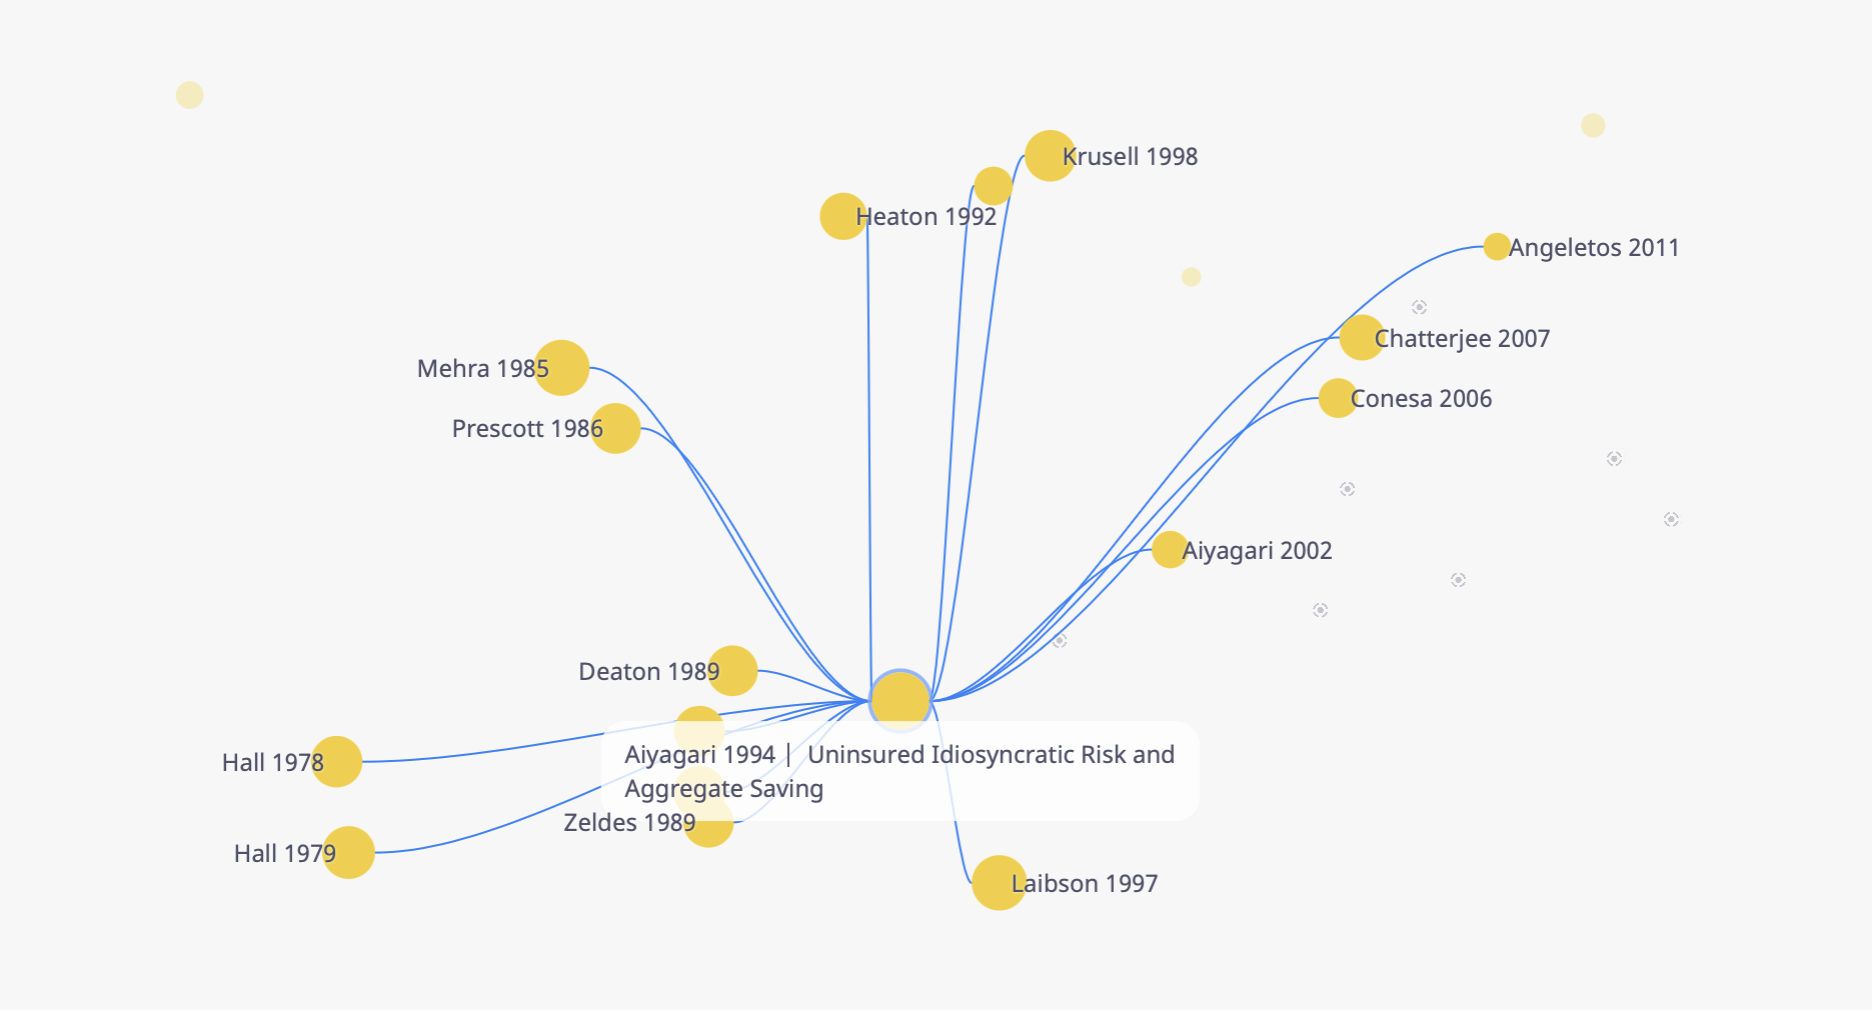
\includegraphics[width=\textwidth]{figures/Exam1.png}

        \vspace*{50mm} % Ensures columns are up top; delete if you want columns centered on page
    \end{column}
    
    \hfill
    
    \begin{column}{.40\textwidth}
        \begin{itemize}
      
            \item Both prior and derivative papers
            \item \textcolor{blue}{Node sizes}: citation
            \item \textcolor{blue}{Edges between nodes}: citation connections
            \item Select/deselect papers to build the graph
            \item Clicking one node shows its connected nodes within the graph 
            \item \href{https://app.litmaps.co/shared/25D4C192-4BA5-4EB9-98C8-2659AB222055}{Link}
        \end{itemize}
    \end{column}
    \end{columns}
    

\end{frame}



\begin{frame}{Example 2}{How are \cite{shiller1989survey} and \cite{kermack_contribution_1927} connected?}
    \begin{columns}[T]
    \vspace{0pt}
    \begin{column}{.60\textwidth}
        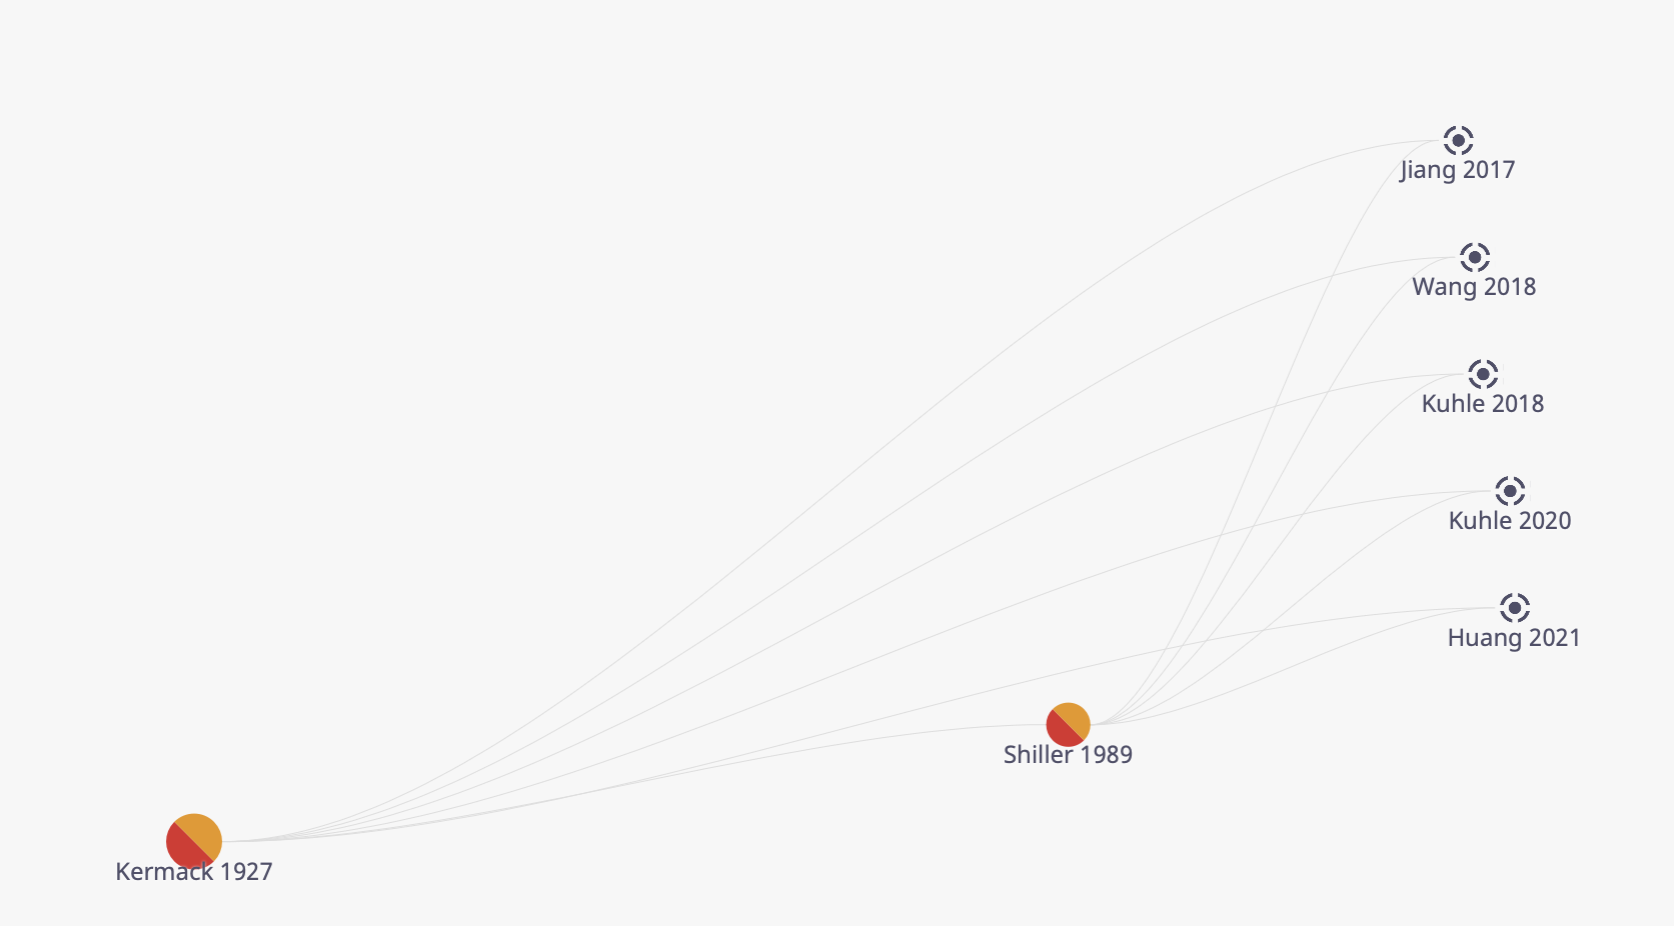
\includegraphics[width=\textwidth]{figures/Exam2.png}

        \vspace*{50mm} % Ensures columns are up top; delete if you want columns centered on page
    \end{column}
    
    \hfill
    
    \begin{column}{.40\textwidth}
        \begin{itemize}
         \item Enter the 2 papers
            \item Choose papers in the suggested list to expand the graph
            \item Real-time algorithms update the suggestions based on your choices
           \item \href{https://app.litmaps.co/shared/7BEBACD2-2307-48D5-91B0-F904C09CD15D}{Link}
        \end{itemize}
        
    \end{column}
    \end{columns}
\end{frame}


\begin{frame}{Example 3}{How are the \textcolor{red}{tech diffusion}, \textcolor{purple}{investors contagion}, and \textcolor{blue}{macroeconomic expectations} literature connected?}
    \begin{columns}[T]
    \vspace{0pt}
    \begin{column}{.60\textwidth}
        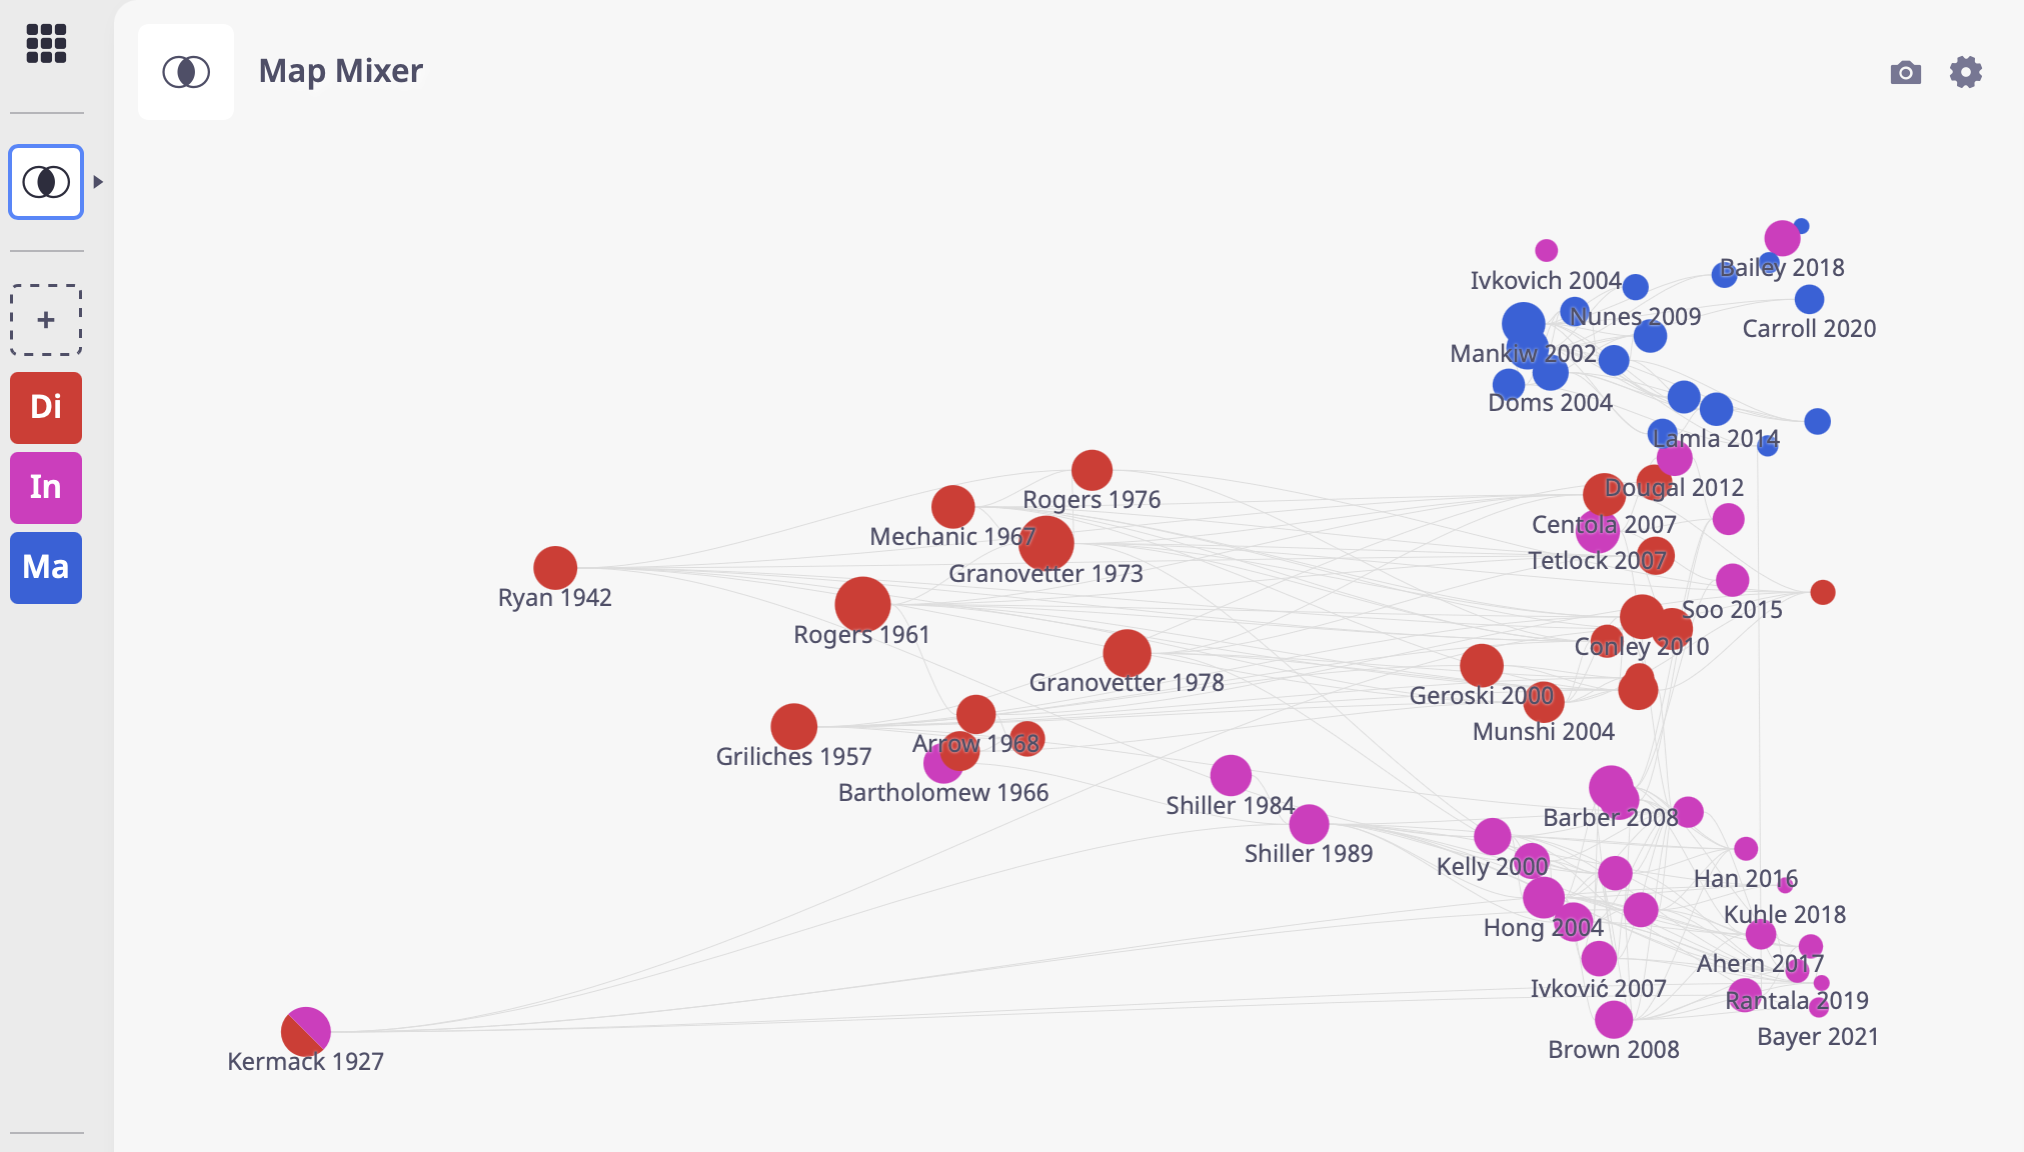
\includegraphics[width=\textwidth]{figures/Exam3.png}

        \vspace*{50mm} % Ensures columns are up top; delete if you want columns centered on page
    \end{column}
    
    \hfill
    
    \begin{column}{.40\textwidth}
        \begin{itemize}
            \item Build separate maps for each topic
            \item Use ``mixer'' function to see if they are connected between each other
            \item  \href{https://app.litmaps.co/shared/0E6D51EB-462D-4F34-8BA2-27925D44DB8F}{Link}
        \end{itemize}
    \end{column}
    \end{columns}
\end{frame}


\begin{frame}{Example 4}{Do I miss any papers in my bibliography? \cite{cw2021epidemiology}}
    \begin{columns}[T]
    \vspace{0pt}
    \begin{column}{.60\textwidth}
        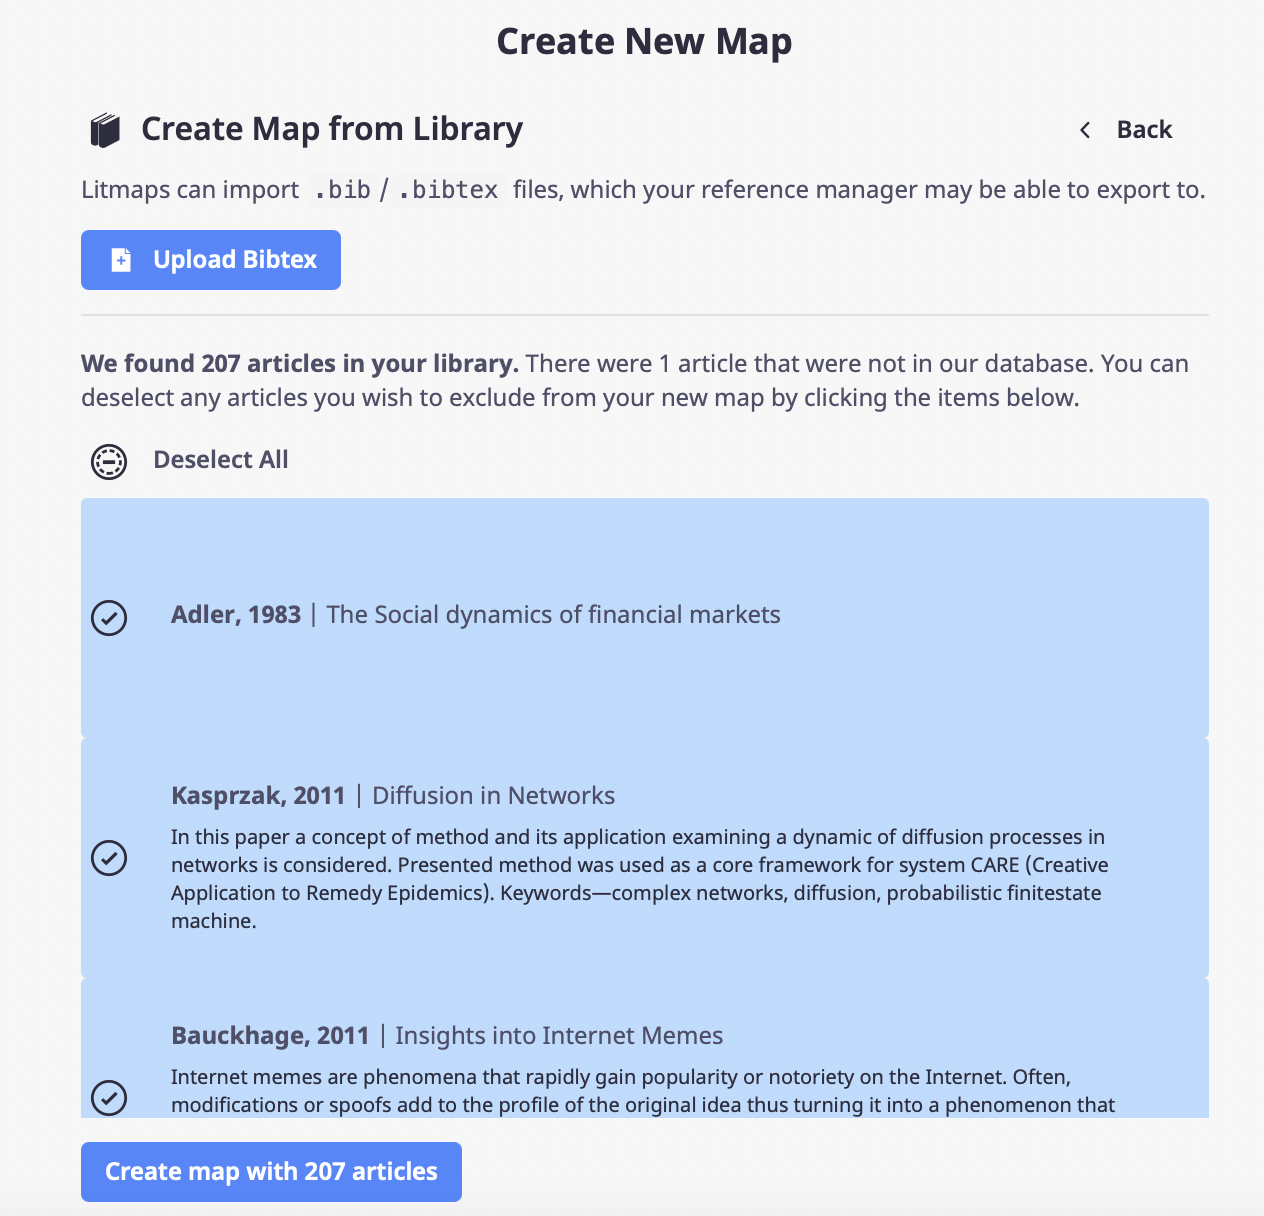
\includegraphics[width=\textwidth]{figures/Exam4.png}

        \vspace*{50mm} % Ensures columns are up top; delete if you want columns centered on page
    \end{column}
    
    \hfill
    
    \begin{column}{.40\textwidth}
        \begin{itemize}
            \item Import your prepared bib file
            \item Exam if there are suggested papers that you should have cited
            \item  \href{https://app.litmaps.co/shared/EC5E5430-1D25-439A-9254-C2025B459D68}{Link}
        \end{itemize}
    \end{column}
    \end{columns}
\end{frame}





\begin{frame}{Other functions}
    
    \begin{itemize}
        \item Import and export bib files: integrated with \LaTeX 
        \item Public sharing: add a link to your website or paper 
        \item Auto updates: keep up-to-date with emerging literature
    \end{itemize}
\end{frame}


% ------------------------------------------------------------------------------
%\begin{frame}[allowframebreaks]{References}
%    \printbibliography
%\end{frame}
% ------------------------------------------------------------------------------

\section{Reference}

\bibliographystyle{apalike}
\bibliography{reference}


\end{document}